%!TEX root = guide2.0.tex

% \section{Summary}\label{sec:PyMCObjects}
Bayesian inference begins with specification of a probability model relating unknown variables to data. PyMC provides three basic building blocks for Bayesian probability models: \texttt{Parameter}, \texttt{Node} and \texttt{Potential}. 

A parameter object represents a variable whose value is not completely determined by its parents, and a node object represents a variable that is determined by its parents. \texttt{Parameter} and \texttt{Node} are subclasses of \texttt{Variable}.

The third basic class, called `potential' or `factor potential' (\cite{dawidmarkov,jordangraphical}), represents an arbitrary log-probability term. This object lends PyMC a great deal of flexibility, but it should be used sparingly if possible. It is most useful in situations where the dependence relationships between variables are not specified. \texttt{Potential} and \texttt{Variable} are subclasses of \texttt{PyMCBase}.

PyMC also provides container classes for parameters and nodes to ease programming of certain dependency situations, such as when a particular variable depends on every element of a Markov chain.

These objects are meant to do perform a small set of behaviors efficiently. As such, they have very limited awareness of the probability model in which they are embedded and no methods for updating their values in an MCMC loop conditional on the rest of the model. PyMC leaves parameter updating functionality to the \texttt{SamplingMethod} class and model-level MCMC supervision to the \texttt{Sampler} class. These objects are described in chapter \ref{chap:modelfitting}. 

Declared probability models can be wrapped in the \texttt{Model} class, which is able to perform model-level tasks such as drawing directed acyclic graphs (\cite{dawidmarkov,jordangraphical}) and computing Bayes factors (\cite{gelman}). \texttt{Sampler} is a subclass of \texttt{Model}.

\section{The \texttt{Variable} classes: \texttt{Parameter} and \texttt{Node}}
Consider the following dataset, which is a time series of recorded coal mining disasters in the UK from 1851 to 1962.
\begin{center}
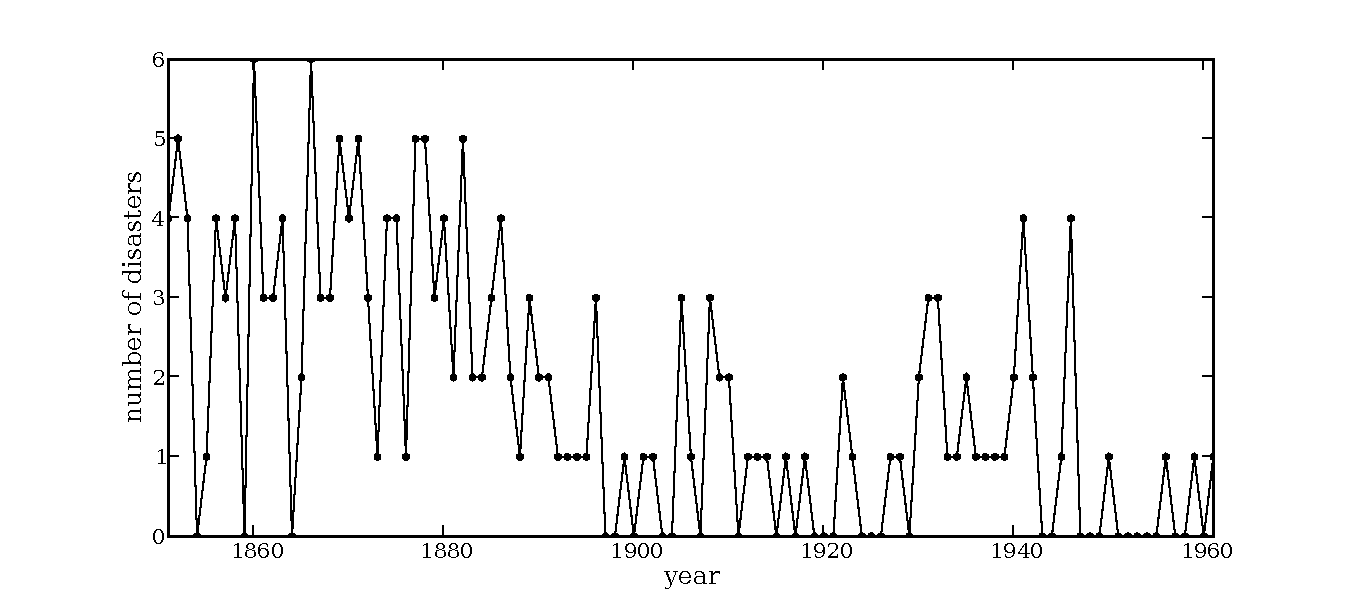
\epsfig{file=disasterts.pdf, width=15cm}
\end{center}
Occurrences of disasters in the time series is thought to be derived from a Poisson process with a large rate parameter in the early part of the time series, and from one with a smaller rate in the later part. We are interested in locating the change point in the series, which perhaps is related to changes in mining safety regulations.

We represent our conceptual model formally as a statistical model:
\begin{equation}
    \begin{array}{ccc}
        (D_t | s, e, l) \sim \textup{Po}\left(r_t\right), & r_t=\left\{\begin{array}{ll}
            e & t\le s\\ l & t>s
            \end{array}\right.,&t\in[1851,1962]\\
        s\sim \textup{U}(t_l, t_h)\\
        e\sim \textup{Exp}(r_e)\\
        l\sim \textup{Exp}(r_l)        
    \end{array}
    \label{disastermodel} 
\end{equation}
The symbols have the following meanings:
\begin{description}
    \item[$D_t$:] The number of disasters in year $t$.
    \item[$r_t$:] The rate parameter of the Poisson distribution of disasters in year $t$.
    \item[$s$:] The year in which the rate parameter changes.
    \item[$e$:] The rate parameter before the switchpoint $s$.
    \item[$l$:] The rate parameter after the switchpoint.
\end{description}
Because $D$ depends directly on $s$, $e$ and $l$, the latter three are known as the \emph{parents} of $D$. $D$ is called the \emph{child} of $s$, $e$ and $l$. Similarly, parents of $s$ are $t_l$ and $t_h$, and $s$ is the child of $t_l$ and $t_h$.

At the model-specification stage (before the data have been observed), $D$, $s$, $e$, $r$ and $l$ are all \emph{random variables}. Under the Bayesian interpretation of probability, `random' variables are not necessarily believed to have arisen from a physical random process. `Random' only means that we are unsure of their values. Random variables are represented in PyMC by class \texttt{Variable}, which has subclasses \texttt{Parameter} and \texttt{Node}.

There is a difference between $r$ and the other variables: if we knew the values of $r$'s parents, we could compute the value of $r$ with no uncertainty. This variable is defined by a mathematical function which returns its value given values for its parents. 

On the other hand, even given values for the parents of $s$ we would still be uncertain of $s$'s value, and similarly for $D$, $e$ and $l$. These variables are defined by probability distributions that express how plausible their candidate values are given values for their parents.
 

\section{The \texttt{Parameter} class}

In PyMC, variables of the latter type are represented by the \texttt{Parameter} class and subclasses. A parameter has two major attributes: \texttt{value}, which gives the parameter's current value, and \texttt{logp}, which gives the log-probability of the parameter's current value given the values of its parents. A parameter can optionally be endowed with a method called \texttt{random}, which draws values for the variable given the values of its parents.

Parameters expose the following additional attributes:
\begin{description}
    \item[\texttt{parents}:] A dictionary containing the parameter's parents. The keys of the dictionary correspond to the names assigned to the parameter's parents by the parameter, and the values correspond to the actual parents. For example, the keys of $s$'s parents dictionary would be \texttt{'t\_l'} and \texttt{'t\_h'}. Since PyMC inherits Python's dynamic typing, parents may be of any class or type.
    \item[\texttt{children}:] A set containing the parameter's children. This set is produced automatically; the user doesn't need to worry about filling it.
    \item[\texttt{isdata}:] A boolean indicating whether the parameter's value has been observed (is fixed).
    \item[\texttt{trace}:] The trace object assigned to the parameter, see chapter \ref{chap:database}.
    \item[\texttt{\_\_name\_\_}:] The name of the parameter, should be unique.
    \item[\texttt{\_\_doc\_\_}:] The docstring of the parameter.
\end{description}

Subclasses of \texttt{Parameter} include the \texttt{DiscreteParameter} class, which represents integer-valued variables, and the \texttt{BinaryParameter} class, which represents Bernoulli or indicator variables. 

\subsection{Instantiation of parameters}
PyMC provides four ways to instantiate parameters, called the `short', `medium', `long' and `direct' interfaces.
\begin{description}
    \item[Short] \textbf{XXX}
    \item[Medium] Uniformly-distributed parameter \texttt{s} could be instantiated using the medium interface as follows:
    \begin{verbatim}
@parameter
def s(value=1900, t_l=1851, t_h=1962):
    """The switchpoint for the rate of disaster occurrence."""
    if value > t_h or value < t_l:
        return -Inf
    else:
        return -log(t_h - t_l) 
    \end{verbatim}
    The decorator \texttt{parameter} turns the function \texttt{s} into a parameter object. This object will evaluate its log-probability using the function \texttt{s}. The \texttt{value} argument, which is required, provides an initial value for the variable. The names of the function's other arguments become the keys of the parameter's \texttt{parents} dictionary, which maps to the corresponding values (parent objects). The name of the function (in this case \texttt{s}) becomes the \texttt{\_\_name\_\_} of the parameter, and the docstring of the function is passed on to the parameter as well.

The parameter may be valued as any object, its parents may be any objects, and there is absolutely no restriction on the log-probability function, as long as it returns a \texttt{float}. Note, however, that PyMC, scientific Python and numerical Python all provide fast implementations of several standard probability distributions.

    The medium interface's decorator can take a flag called \texttt{trace} which signals to \texttt{Model} whether an MCMC trace should be kept for the parameter: \texttt{@parameter(trace = False)} would turn tracing off.

    \item[Long] The long interface extends the medium interface by allowing the user to specify a method for sampling the parameter's value conditional only on its parents.
    \begin{verbatim}
@parameter
def s(value=1900, t_l=1851, t_h=1962):
    """The switchpoint for the rate of disaster occurrence."""

    def logp(value, t_l, t_h):
        if value > t_h or value < t_l:
            return -Inf
        else:
            return -log(t_h - t_l) 
            
    def random(t_l, t_h):
        return round( (t_l - t_h) * random() ) + t_l

    rseed = 1.
    \end{verbatim}
The parameter again gets its name, docstring and parents from function \texttt{s}, but in this case it will evaluate its log-probability using the \texttt{logp} function. The \texttt{random} function will be used when \texttt{s.random()} is called. Note that it doesn't take a \texttt{value} argument, because it provides a new value. \textbf{XXX David explain rseed} \texttt{rseed} provides a seed for the RNG. The \texttt{value} argument is optional if a \texttt{random} method is provided; if no initial value is provided, it will be drawn using the \texttt{random} method.

    \item[Direct] Some users may prefer not to use the \texttt{@parameter} decorator, but to instantiate \texttt{Parameter} directly:
\begin{verbatim}
def s_logp(value, t_l, t_h):
    if value > t_h or value < t_l:
        return -Inf
    else:
        return -log(t_h - t_l) 

def s_rand(t_l, t_h):
    return round( (t_l - t_h) * random() ) + t_l

s = Parameter(logp = s_logp, 
name = 's', 
value = 1900,
parents = {'t_l': 1851, 't_h': 1962},
doc = 'The switchpoint for the rate of disaster occurrence.',
random = s_rand, 
trace = True, 
rseed = 1., 
isdata = False,
cache_depth = 2)
\end{verbatim}
\end{description}

\subsection{Don't update parameters' values in-place}

\texttt{Parameter} objects' values should not be updated in-place. This would confuse the cache checker and destroy the `last value' attribute of the parameter, which is used for rejecting jumps. The only way a parameter's value should be updated is using statements of the following form:
\begin{verbatim}
    A.value = new_value
\end{verbatim}
where \texttt{new\_value} is an object that has just been created for this purpose. The following should \emph{not} be used:
\begin{itemize}
    \item \texttt{A.value += 3}. This is an in-place update if $A$'s value is a numpy array.
    \item \texttt{A.value[2,1] = 5}. This is an in-place update also if $A$'s value is a numpy array.
    \item \texttt{A.value.attribute = new_attribute_value}. This is an in-place update regardless of what type of object \texttt{A.value} is.
\end{itemize}


\section{Data}

Although $D$ was a random variable at the model-specification stage, we subsequently observed its value by looking at the data. In PyMC such variables are represented by \texttt{Parameter} objects whose \texttt{isdata} attribute is set to \texttt{True}. If a parameter's \texttt{isdata} flag is \texttt{True}, its value cannot be changed.

\subsection{Why are data and unknown parameters represented by the same object?}
Since it's represented by a \texttt{Parameter}, $D$ formally depends on $s$, $e$ and $l$ even though its value is fixed. This isn't just a quirk of PyMC's syntax; Bayesian hierarchical notation itself makes no distinction between unobserved random variables (parameters) and observed random variables (data). This point can be counterintuitive at first, as most scientists' instinct is to regard data as fixed a priori and unknown parameters' values as dependent on the data. The value of data is fixed, after all, so how could it depend on anything?

One way to understand this issue is to think of statistical models like (\ref{disastermodel}) as predictive models for data, or as models of the processes that gave rise to data. Before observing the value of $D$, we could have easily sampled from its prior predictive distribution $p(D)$ as follows:
\begin{enumerate}
    \item Sample $e$, $s$ and $l$ from their priors.
    \item Sample $D$ conditional on these values.
\end{enumerate}
Even after we observe the value of $D$, we need to use this process model to make inferences about $e$, $s$ and $l$.

\medskip
To look at the issue another way, we could in principle have written a model equivalent to (\ref{disastermodel}) in such a way that $D$ depended on nothing and everything else depended on $D$, for example
\begin{eqnarray*}
    s|e,l,D\sim\cdot\\
    e|l,D\sim\cdot\\
    l|D\sim\cdot\\
    D\sim\cdot
\end{eqnarray*}

This would have felt more natural in some ways, because we would have the unknown parameters depending on the data. However, if we could write down that model using standard distributions we could trivially compute and sample from the posterior density,
\begin{eqnarray*}
    p(s,e,l|D) = p(s|e, l, D) p(e|l, D) p(l|D),
\end{eqnarray*}
and we would have no use for MCMC or any other fitting method. Bayesian methods, and statistics in general, are needed when it's more natural to model the data as depending on the unknown parameters than vice versa.

\subsection{Declaring parameters to be data}

In the medium and long interfaces, a \texttt{Parameter} object's \texttt{isdata} flag can be set to true by stacking a \texttt{@data} decorator on top of the \texttt{@parameter} decorator:
\begin{verbatim}
@data
@parameter
def D(value = count_array, switchpoint = s, early_rate = e, late_rate = l):
    """The observed annual disaster counts."""
    logp = sum(-value[:switchpoint]) + early_rate * log(value[:switchpoint]) - gammaln(early_rate))
    logp += sum(-value[switchpoint:] + late_rate * log(value[switchpoint:]) - gammaln(late_rate))
    return logp
\end{verbatim}
In the direct interface, the \texttt{isdata} argument can be simply set to \texttt{True}.


\section{The \texttt{Node} class}\label{node}

Nodes represent variables whose values are fully determined by the values of their parents. The variables on which a node's value depends are called the parents of the node, as with parameters. In model (\ref{disastermodel}), $r$ can be represented as a node. Recall that $r_t$ was defined by
\begin{eqnarray*}
    r_t=\left\{\begin{array}{ll}
        e & t\le s\\ l & t>s
        \end{array}\right.,
\end{eqnarray*}
so $r$'s value can be computed from the values of its parents $e$, $l$ and $s$.

A node's most important attribute is called \texttt{value}, and gives the current value of the node given the values of its parents. Like \texttt{Parameter}'s \texttt{logp} attribute, this attribute is computed on-demand and cached for efficiency.

Nodes expose the following additional attributes:
\begin{description}
    \item[\texttt{parents}:] A dictionary containing the node's parents. The keys of the dictionary correspond to the names assigned to the node's parents by the node, and the values correspond to the actual parents. Since PyMC inherits Python's dynamic typing, parents may be of any class or type.
    \item[\texttt{children}:] A set containing the node's children, which must be parameters or nodes. This set is produced automatically; the user doesn't need to worry about filling it.
    \item[\texttt{trace}:] The trace object assigned to the node, see chapter \ref{chap:database}.
    \item[\texttt{\_\_name\_\_}:] The name of the node, should be unique.
    \item[\texttt{\_\_doc\_\_}:] The docstring of the node.
\end{description}
Nodes have no methods.

\subsection{Nodes are optional}
If we make a node out of $r$, we'll want to rewrite $D$ as follows:
\begin{verbatim}
@data
@parameter
def D(value=count_array, rate=r):
    """The observed annual disaster counts."""
    return sum(-value + rate * log(value) - gammaln(rate))
\end{verbatim}
It's up to us whether to use $r$ or to leave it out of the model: use of the node class is always optional. However, nodes can be nice for the following reasons:
\begin{itemize}
    \item They can save code duplication,    
    \item they can be computationally efficient (because they save code duplication), and
    \item sometimes it's convenient to produce a dynamic trace of the value of a function of parameters.
\end{itemize}


\subsection{Instantiation of nodes}
Nodes are less complicated than parameters, and PyMC provides only two ways to instantiate them:
\begin{description}
    \item[Decorator] A node can be instantiated via a decorator in a way very similar to parameter's medium interface:
\begin{verbatim}
@node
def r(switchpoint = s, early_rate = e, late_rate = l):
    """The rate of disaster occurrence."""
    value = zeros(N)
    value[:switchpoint] = early_rate
    value[switchpoint:] = late_rate
    return value
\end{verbatim}
The function supplied should return a new value (which may be any object) for the node. Arguments' keys and values are converted into a parent dictionary as with parameter's medium interface. The function's \texttt{\_\_name\_\_} is passed on to the node.
    \item[Direct] The same node could be instantiated directly as follows:
\begin{verbatim}
def r_eval(switchpoint = s, early_rate = e, late_rate = l):
    value = zeros(N)
    value[:switchpoint] = early_rate
    value[switchpoint:] = late_rate
    return value

r = Node(eval = r_eval, 
name = 'r',
parents = {'switchpoint': s, 'early_rate': e, 'late_rate': l}),
doc = 'The rate of disaster occurrence.',
trace = True,
cache_depth = 2)
\end{verbatim}
The \texttt{trace} flag signals to \texttt{Model} whether to keep a trace for self, as with parameter.
\end{description}

Note that nodes have no \texttt{isdata} flag. If a node's value were known, its parents would be restricted to the inverse image of that value under the node's evaluation function. This usage case would be extremely difficult to support in generality, but it can be implemented for particular applications at the \texttt{SamplingMethod} level.

\section{Using \texttt{Variables} as parents of \texttt{Variables}}

Let's take a closer look at our most recent definition of $D$:
\begin{verbatim}
@data
@parameter
def D(value=count_array, rate=r):
    """The observed annual disaster counts."""
    return sum(-value + rate * log(value) - gammaln(rate))
\end{verbatim}
The value of argument \texttt{rate} is a \texttt{Node} object, not a number. Why aren't errors raised when we attempt to multiply \texttt{rate} by an array?

Whenever a variable is used as a parent for a child variable, it is replaced with its \texttt{value} attribute when the child's value or log-probability is computed. So when $D$'s log-probability is recomputed, \texttt{r.value} is passed to the function as argument \texttt{rate}. 

\section{Containers}\label{sub:container}
In the following situation, it would be inconvenient to assign a unique label to each parent of $y$:
\begin{eqnarray*}
    x_0 \sim \textup N(0,\tau_x)\\
    x_{i+1}|x_i\sim\textup{N}(x_i, \tau_x),& i=0\ldots N-2\\
    y|x \sim \textup N\left(\sum_{i=0}^{N-1}x_i^2,\tau_y\right).
\end{eqnarray*}
$y$ depends on every element of the Markov chain $x$, but we wouldn't want to manually enter $N$ parent labels \texttt{'x_0'}, \texttt{'x\_1'}, etc.

This situation can be handled using the \texttt{Container} function as follows:
\begin{verbatim}
@parameter
def x_0(value=0, mu = 0, tau = 1):
    return normal_like(value, mu, tau)

x_list = [x_0]
last_x = x_0

for i in range(1,N):          
    @parameter
    def x_now(value=0, mu = last_x, tau = 1):
        return normal_like(value, mu, tau)
    x_now.__name__ = 'x\_%i' % i
    last_x = x_now
    
    x_list.append(x_now)
        
x = Container(x_list, name = 'x')

@data
@parameter
def y(value = 1, mu = x, tau = 100):
    mu_sum = 0
    for i in range(N):
        mu_sum += mu[i] ** 2
    return normal_like(value, mu_sum, tau)
\end{verbatim}
The \texttt{Container} function wraps \texttt{x\_list} in an appropriate PyMC container class and returns it.

Containers, like parameters and nodes, expose an attribute called \texttt{value}. This attribute returns a copy of the (possibly nested) iterable that was passed into the container function, but with each instance of a parameter or node inside replaced with \emph{its} value. Note that simply writing
\begin{verbatim}
@data
@parameter
def y(value = 1, mu = x_list, tau = 100):
    mu_sum = 0
    for i in range(N):
        mu_sum += mu[i] ** 2
    return normal_like(value, mu_sum, tau)
\end{verbatim}
would not have worked, because \texttt{list} does not expose an attribute called \texttt{value}. 

PyMC containers can currently be constructed from any object that has a \texttt{\_\_getitem\_\_} method (such as lists, tuples and dictionaries), numpy arrays, and sets. Variables and non-variables can be freely mixed in these iterables, and different types of iterables can be nested. Containers attempt to behave like the iterables they wrap, but are read-only. All containers are subclasses of \texttt{ContainerBase}.

Containers have the following useful attributes in addition to \texttt{value}:
\begin{itemize}
    \item\texttt{variables}
    \item\texttt{parameters}
    \item\texttt{potentials}
    \item\texttt{nodes}
    \item\texttt{data}
    \item\texttt{all_objects}
    \item\texttt{sampling_methods}.
\end{itemize}
Each of these attributes is a set containing all the objects of each type in a container, and within any containers in the container.

\section{The \texttt{Potential} class}

The joint density corresponding to model (\ref{disastermodel}) can be written as follows:
\begin{eqnarray*}
    p(D,s,l,e) = p(D|s,l,e) p(s) p(l) p(e).
\end{eqnarray*}
Each factor in the joint density is a proper, normalized probability density for one of the variables conditional on its parents. Such factors are contributed by \texttt{Parameter} objects.

In some cases, it's nice to be able to modify the joint density by incorporating terms that don't correspond to probabilities of variables conditional on parents, for example:
\begin{eqnarray*}
    p(D,s,l,e) \propto \chi(D,s,e) p(D|s,l,e) p(s) p(l) p(e),
\end{eqnarray*}
or
\begin{eqnarray*}
    p(D,s,l,e) \propto \psi(D,s,l,e) p(s) p(l) p(e).
\end{eqnarray*}
Arbitrary factors such as $\psi$ and $\chi$ are contributed by objects of class \texttt{Potential} (\cite{dawidmarkov} and \cite{jordangraphical} call these terms `factor potentials'). Bayesian hierarchical notation doesn't accomodate potentials, possibly because models involving potentials are a little strange:
\begin{itemize}
    \item The term $p(D|s,l,e)$ no longer gives the density of $D$ conditional on its parents.
    \item Densities constructed using potentials are usually not normalized, which complicates computation of Bayes' factors.
    \item The Bayesian interpretation of probability theary can be viewed as an extension of propositional logic: propositions such as `if $x=3$ then $y=2$' give way to probabilistic statements such as `if $x=3$ then $y\sim\textup N(2,V)$'. \cite{jaynes} gives an intuitive explanation of Cox's theorem, which says that probability theory is the only `logic of uncertainty' that satisfies a three very sensible desiderata. Potentials blur the hierarchical dependence structure of models, and with it the logical interpretation of the model.
\end{itemize}
However, potentials are useful for cases where there is no clear dependence structure, especially Markov random fields \textbf{CITE} and models of random graphs (\cite{durrettrandomgraph}). See section \ref{sec:graphical}.

Even when there is a definite dependence structure, potentials can provide a useful shorthand. Consider a new example: we have a dataset $t$ consisting of the days on which several marked animals were recaptured. We believe that the probability $S$ that an animal is not recaptured on any given day can be explained by a covariate vector $x$. We model this situation as follows:
\begin{eqnarray*}
    t_i|S_i \sim \textup{Geometric}(S_i), & i=1\ldots N\\
    S_i = \textup{logit}^{-1}(\beta x_i), &i=1\ldots N\\
    \beta\sim \textup{N}(\mu_\beta, V_\beta).
\end{eqnarray*}
So far, so good. Now suppose we have some knowledge of other related experiments and we have a good idea of what $S$ will be before seeing the data. It's not obvious how to work this prior information in, because as we've written the model $S$ is completely determined by $\beta$. There are three equally unpalatable options within the strict Bayesian hierarchical framework:
\begin{itemize}
    \item Work the prior information into the prior on $\beta$.
    \item Incorporate the data from the previous experiments explicitly into the model.
    \item Refactor the model so that $S$ is at the bottom of the hierarchy, and assign the prior directly.
\end{itemize}

Potentials provide a convenient way to incorporate the prior information without the need for such major modifications. We can simply modify the joint distribution from
\begin{eqnarray*}
    p(t|S(x,\beta)) p(\beta)
\end{eqnarray*}
to
\begin{eqnarray*}
    \gamma(S,a,b) p(t|S(x,\beta)) p(\beta),
\end{eqnarray*}
where $\gamma$ expresses the prior information. It's a good idea to check the induced priors on $S$ and $\beta$ for sanity. This can be done in PyMC by fitting the model with the data $t$ commented out.

\bigskip
Potentials have one important attribute, \texttt{logp}, which gives the log their current probability value given the values of their parents. They expose the following additional attributes:
\begin{description}
    \item[\texttt{parents}:] A dictionary containing self's parents. The keys of the dictionary correspond to the names assigned to the potential's parents by the potential, and the values correspond to the actual parents. Since PyMC inherits Python's dynamic typing, parents may be of any class or type.
    \item[\texttt{\_\_name\_\_}:] The name of the potential, should be unique.
    \item[\texttt{\_\_doc\_\_}:] The docstring of the potential.
\end{description}
Potentials have no methods. They have no \texttt{trace} attribute, because they are not variables. They cannot serve as parents of variables for the same reason, so they have no \texttt{children} attribute.


\subsection{Instantiation of potentials}
PyMC provides two ways to instantiate potentials:
\begin{description}
    \item[Decorator] A potential can be instantiated via a decorator in a way very similar to parameter's medium interface and node's decorator interface:
\begin{verbatim}
@potential
def gamma(surv_rate = S, a = a, b = b):
    """Some random potential."""
    return beta_like(surv_rate, a, b)
\end{verbatim}
The function supplied should return a floating-point value. Arguments' keys and values are converted into a parent dictionary as with parameter's medium interface. The function's \texttt{\_\_name\_\_} is passed on to the potential.
    \item[Direct] The same potential could be instantiated directly as follows:
\begin{verbatim}
def gamma_logp    (surv_rate = S, a = a, b = b):
        return beta_like(surv_rate, a, b)
        
gamma = Potential(logp = gamma_logp, 
name = 'gamma',
parents = {'surv_rate': S, 'a': a, 'b': b}),
doc = 'Prior information for S.',
cache_depth = 2)
\end{verbatim}
\end{description}

\section{Graphical models (optional)}
\label{sec:graphical}

It's often helpful to view probability models graphically; graphical representations harmonize very well with object-oriented programming, so most Bayesian statistics packages (including PyMC) are at least somewhat graphically inspired. PyMC's \texttt{Model} object provides a method called \texttt{graph} which converts PyMC models to graphical models using GraphViz. See \cite{dawidmarkov} and \cite{jordangraphical} for more discussion of useful information that can be read off of graphical models. Note that these authors do not consider nodes.

PyMC's symbol for parameters is the ellipse. Parent-child relationships are indicated by arrows. These arrows always point from parent to child, and PyMC labels them with the names assigned to the parents by the children. A graphical representation of model \ref{disastermodel} follows:
\begin{center}
    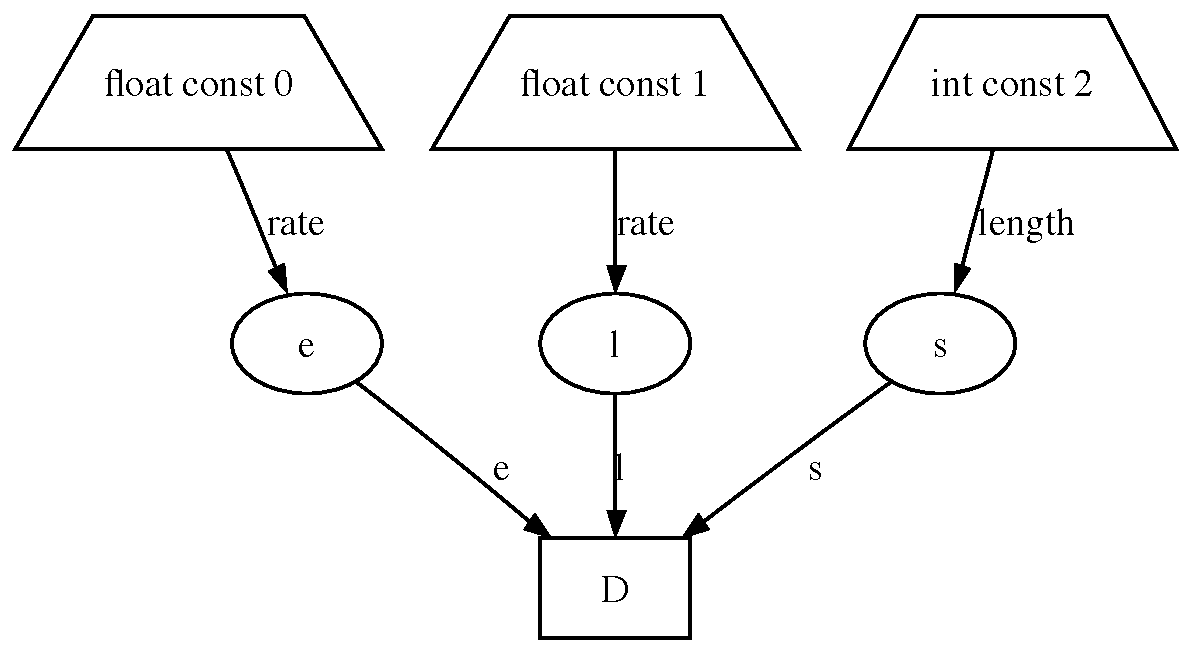
\epsfig{file=DisasterModel.pdf, width=6cm} 
\end{center} 
$D$ is shaded because it is flagged as data.

PyMC's symbol for nodes is a downward-pointing triangle. A graphical representation of model \ref{disastermodel} with $r$ explicit follows:
\begin{center}
    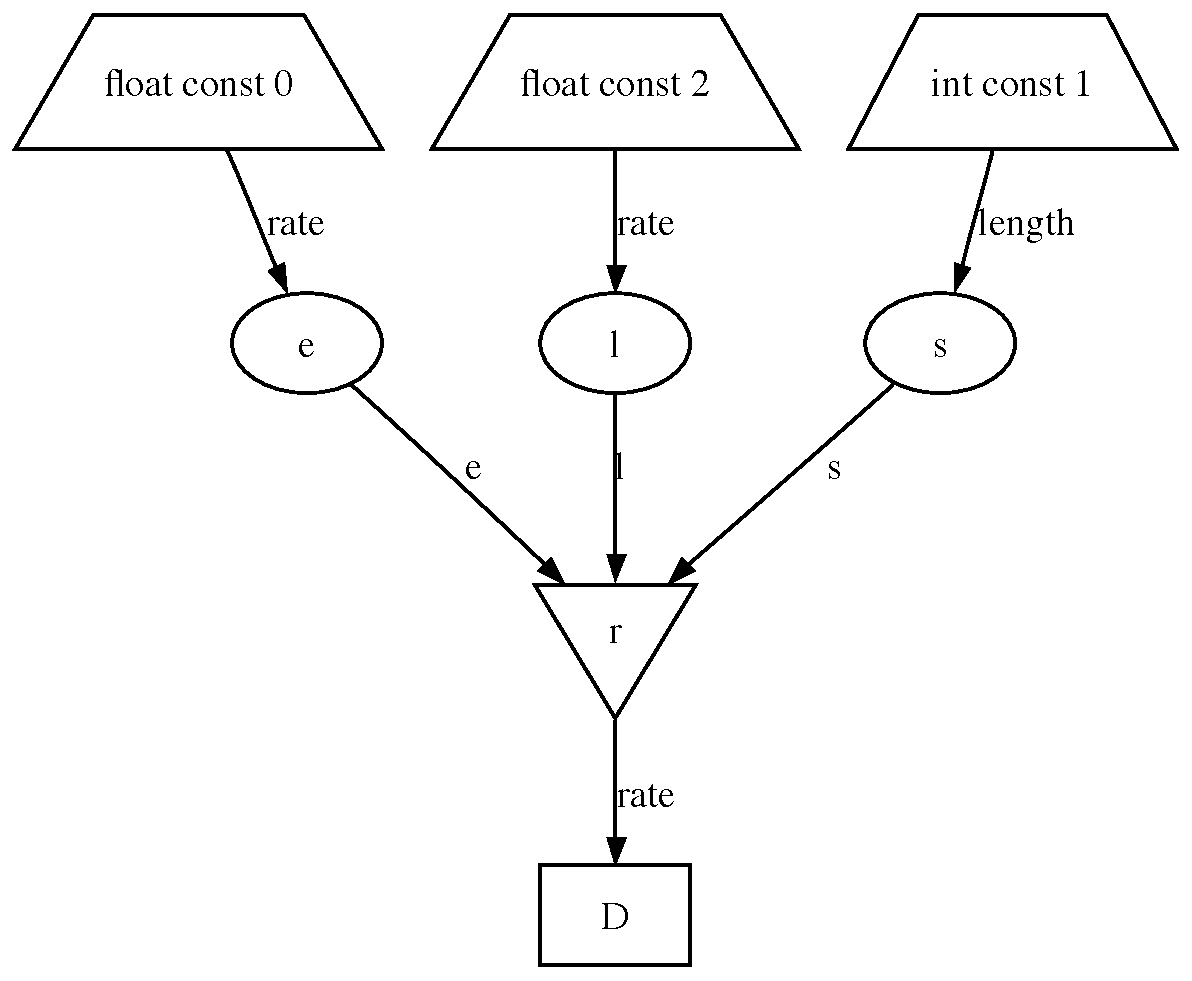
\epsfig{file=DisasterModel2.pdf, width=6cm} 
\end{center}
Note that if a node has more than one child, its parents each inherit all of its children when it is made implicit:
\begin{center}
    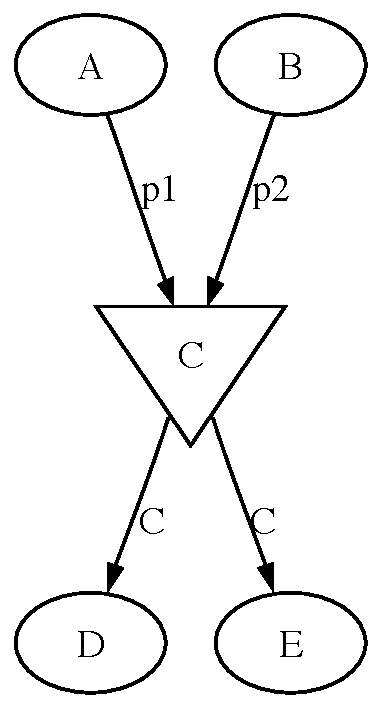
\epsfig{file=NodePreInheritance.pdf, width=3.5cm} \textbf{XXX How can I move this arrow up?} $\Rightarrow$ 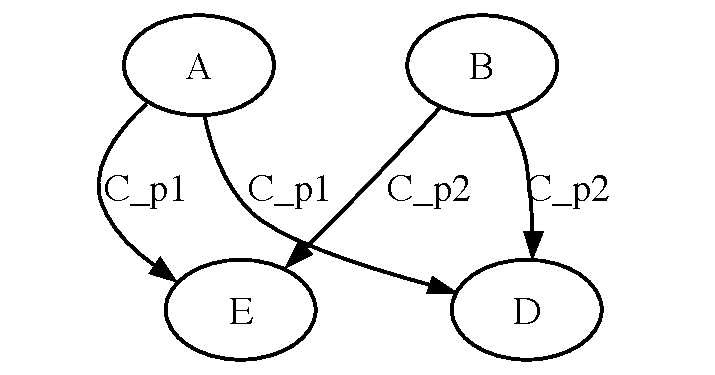
\epsfig{file=NodePostInheritance.pdf, width=5cm}
\end{center}
Incidentally, these inherited children can be found using the function \texttt{extend\_children} provided by PyMC. Sampling method objects use this function to evaluate the log-likelihoods of the parameters they handle.

PyMC's symbol for potentials is a triple-outlined octagon:
\begin{center}
    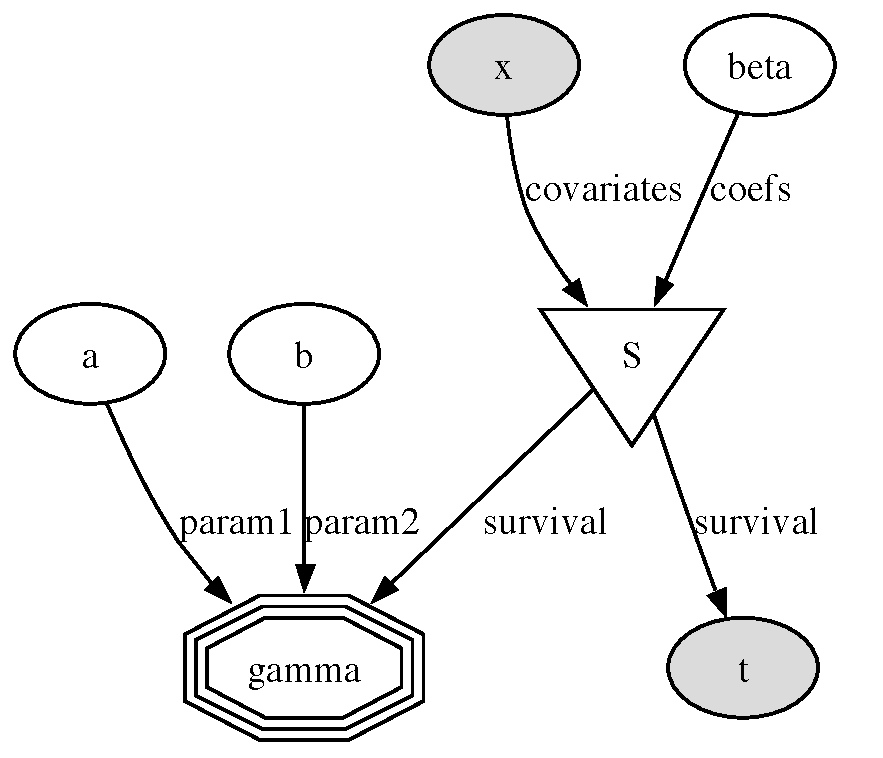
\epsfig{file=SurvivalModel.pdf, width=6cm} 
\end{center}
Potentials are usually associated with \emph{undirected} grahical models. In undirected representations, each parent of a potential is connected to every other parent by an undirected edge:
\begin{center}
    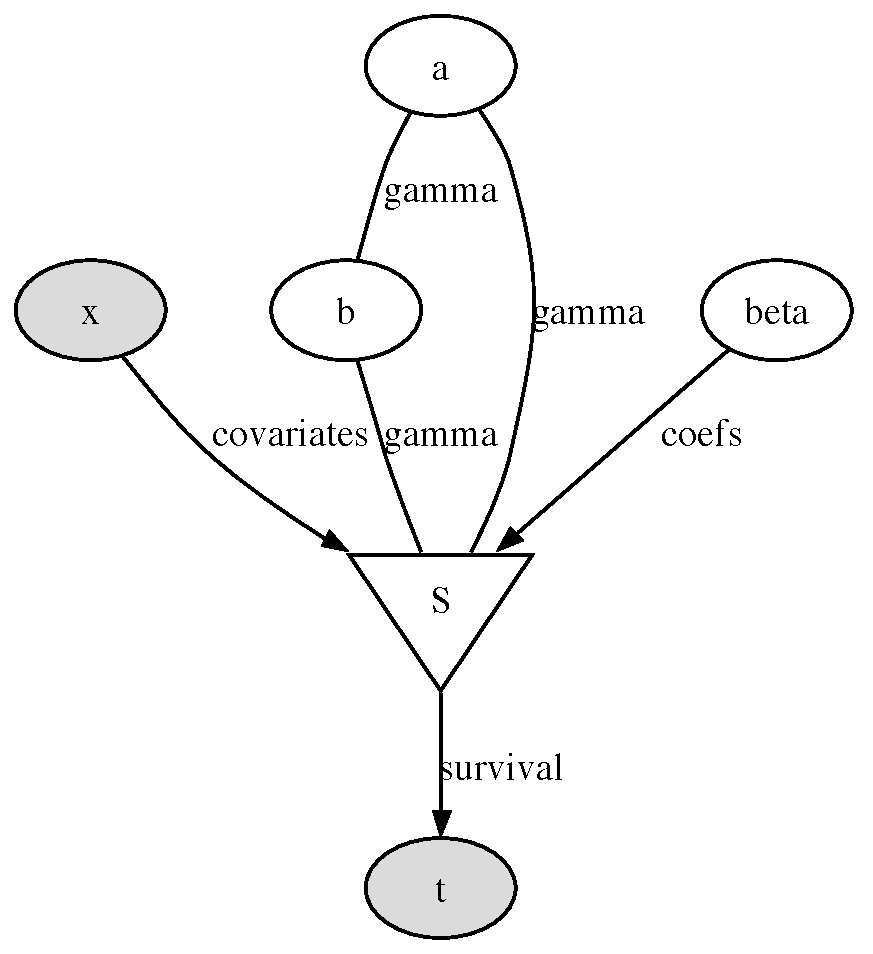
\epsfig{file=SurvivalModelCollapsed.pdf, width=5cm}
\end{center}
Mixing undirected and directed edges in the same model can be confusing, but fortunately the technique of \emph{moralization} can convert directed edges to undirected.

\cite{dawidmarkov} and \cite{jordangraphical} give several results on conditional independence and dependence that can be obtained just from looking at the structure of a graphical model, without knowing the forms of the probability distributions involved at all. A particularly important concept is $d$-separation, which indicates when a group of parameters $A$ will be independent of another group $B$ given a third group $S$.

\section{LazyFunction (optional)}
\subsection{Caching}  
\label{sec:caching}

% \section{Graphical models}
% 
% The dependence structure of a statistical model can be represented by a \emph{directed acyclic graph}. For our coal-mining disaster model, the PyMC-generated DAG is illustrated in figure \ref{fig:disasterdag}. The arrows in the figure point from parent to child, or alternatively from antecedent to consequent.
% 
% In principle, we could have written down other statistical models that gave the same joint distribution (and hence the same posterior distribution). For example, we could have specified the model as
% \begin{eqnarray*}
% p(s|D,l,e)\prod_tp(D_t|l,e,D_{1851\ldots t-1})p(l)p(e),
% \end{eqnarray*}
% and drawn a new DAG representation of the dependence structure. However, that would have been extremely uncomfortable. Our intuition tells us that $e$, $l$ and $s$ influence $D_t$, not that $D_t$, $e$ and $l$ influence $s$. In other words, the statement
% \begin{quote}
% Given the rate parameter before the switchpoint, the rate parameter after the switchpoint, and the switchpoint itself, the distribution of disasters in year $t$ is $d$.
% \end{quote}
% is much more natural than the statement
% \begin{quote}
% Given the rate parameter befare the switchpoint, the rate parameter after the switchpoint, and annual disasters up to year $t-1$, the distribution of disasters in year $t$ is $d^*$. Further, given all the data on annual disasters the distribution of the switchpoint is $d^{**}$.
% \end{quote}
% 
% \begin{figure}[hhhhhhhhhhh]
% \begin{center}
% 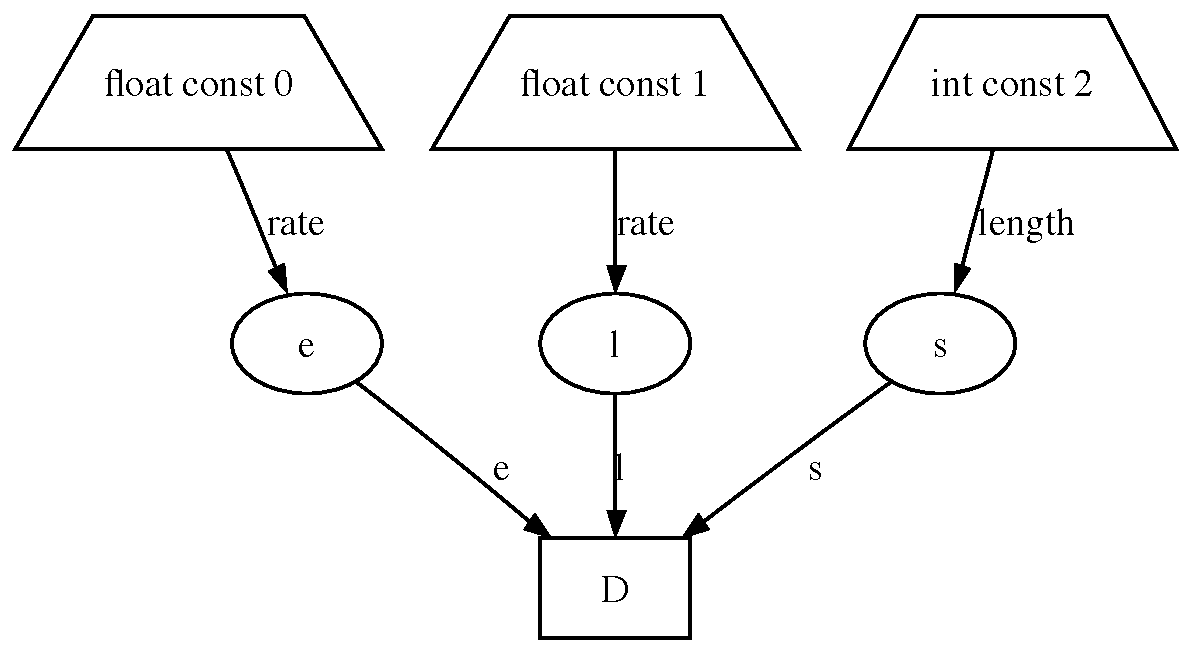
\epsfig{file=DisasterModel.pdf,width=7cm}
% 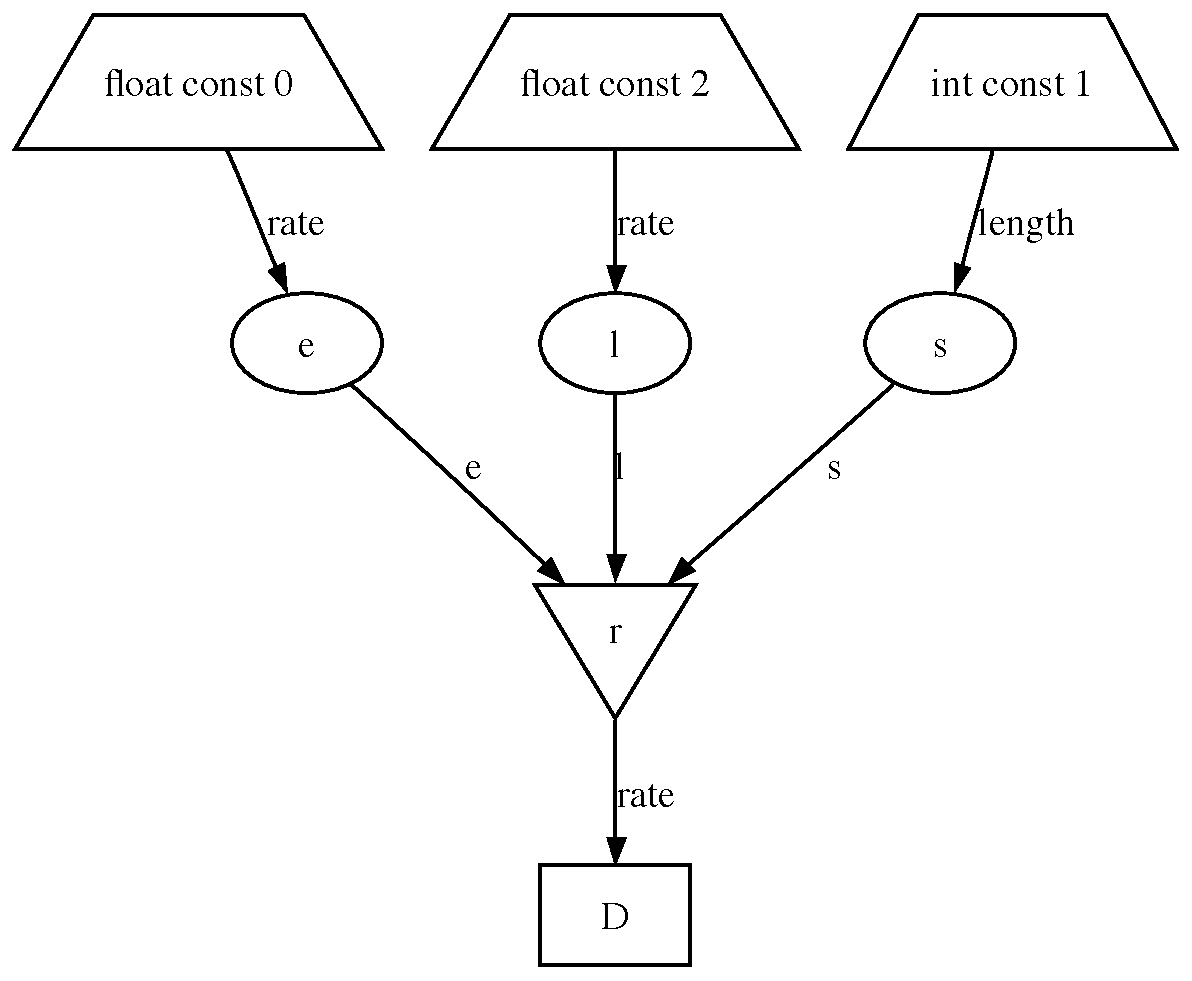
\epsfig{file=DisasterModel2.pdf,width=7cm}
% \caption{\textbf{Left:} A DAG of the coal-mining disaster example with the function $r_t$ implicit. \textbf{Right:} An equivalent DAG with $r_t$ explicit. The `float const's refer to the parameters of the priors of $e$, $l$ and $s$. The labels on the arrows refer to the parameter names assigned to the parents by the child. For example, in the DAG on the right $D$ considers $r$ to be its `rate' parameter.
% }
% \label{fig:disasterdag}
% \end{center}
% \end{figure}


\section{The \texttt{Model} class} \label{sec:Model}
This class serves as a container for probability models and as a stem class for other `model-level' classes like \texttt{Sampler}. Methods implemented:
\begin{description}
    \item[\texttt{sample\_model\_likelihood(\texttt{iter})}:] Returns \texttt{k} samples from $\log p(d_M|\theta_M, M)$, the log-probability or log-density of all the data $d_M$ in model $M$ given all the parameters $\theta_M$. This is called by the function \texttt{weight()}, which finds the Bayes factors for a set of models.
    \item[\texttt{graph()}:] \textbf{XXX}
    \item[\texttt{tally()}:] Tells all parameters and nodes to record their current values in their traces.
    \item[\texttt{remember(trace\_index)}:] Tells all parameters to revert to a certain index from their traces.
    \item[\texttt{status():}] \textbf{XXX}
    \item[\texttt{save\_traces(path, fname)}:] \textbf{XXX}
    \item[\texttt{seed()}:] \textbf{XXX}
\end{description}

Useful set attributes:
\begin{enumerate}
    \item \texttt{containers}
    \item \texttt{parameters}
    \item \texttt{nodes}
    \item \texttt{variables}
    \item \texttt{potentials}
    \item \texttt{data}
\end{enumerate}



\subsection{Examples}\label{sub:example}
Here is the coal-mining disaster model implemented in PyMC with $r$ implicit, as in the left pane of figure \ref{fig:disasterdag}:
\begin{verbatim}
@parameter
def s(value=50, length=110):
    """Change time for rate parameter."""
    constrain(value, 0, length)
    return 0.

@parameter
def e(value=1., rate=1.):
    """Rate parameter of poisson distribution."""
    return exponential_like(value, rate)

@parameter
def l(value=.1, rate = 1.):
    """Rate parameter of poisson distribution."""
    return exponential_like(value, rate)

@data
def D(  value = D_array,
        switchpoint = s,
        early_mean = e,
        late_mean = l):
    """Annual occurences of coal mining disasters."""
    return poisson_like(value[:s],e) + poisson_like(value[s:],l)
\end{verbatim}
To make $r$ explicit as in the right pane of figure \ref{fig:disasterdag}, we would write:
\begin{verbatim}
@parameter
def s(value=50, length=110):
    """Change time for rate parameter."""
    constrain(value, 0, length)
    return 0.

@parameter
def e(value=1., rate=1.):
    """Rate parameter of poisson distribution."""
    return exponential_like(value, rate)

@parameter
def l(value=.1, rate = 1.):
    """Rate parameter of poisson distribution."""
    return exponential_like(value, rate)

@node
def r(l=l,e=e,s=s):
    """r = function(l,e,s)"""
    ret_val =  ones(111,dtype=float)
    ret_val[:s] = e
    ret_val[s:] = l
    return ret_val

@data
def D(  value = D_array, rate=r):
    """Annual occurences of coal mining D."""
    return poisson_like(value,rate)
\end{verbatim}
In general, it's better to make heavyweight functions into their own nodes, because nodes' caches avoid unnecessary recomputation. In this case, however, the version with $r$ implicit is quite a bit faster.